\chapter{Metodologia}
Dado os conceitos que envolve a diferença de desempenho entre a paravirtualização e a virtualização total e os problemas relacionados a interferência entre máquinas virtuais, neste capítulo serão definidas as abordagens que irão dar norte para o desenvolvimento destre trabalho. Desse modo, em um primeiro momento são apresentado os trabalhos relacionados à análise de desempenho em ambientes virtuais, de modo que é definida a abordagem mais adequada para o estudo de caso do LAPPIS. Em seguida são definidas as hipóteses, a partir de uma questão problema, que irão conduzir este trabalho. Por fim, são apresentados as espeficiações voltadas para ambientes de testes , coleta de dados e análise de dados.
\section{Trabalhos relacionados}
Essa seção tem como intuito expor alguns trabalhos relacionados à análise de desempenho. Esses trabalhos também servirão de insumo para desenvolvimento do estudo de interferência de desempenho proposto por este trabalho.

No trabalho apresentado por \cite{koh2007} é feito um estudo de interferência entre aplicações executadas sobre o mesmo \textit{hardware} a partir de máquinas virtuais. Como cargas de trabalho, foram escolhidas aplicações do mundo real utilizadas para compressão, compilação de código fonte, e renderização de \textit{frames}, bem como fora utilizadas ferramentas voltadas para testes de desempenho (\textit{benchmark}).

\begin{table}[!h]
\centering
%\cite{koh2007}
\caption{Aplicações utilizadas para testes de desempenho \cite{koh2007}.}
\label{applications}
\resizebox{0.6\textwidth}{!}{
\begin{tabular}{|l|c|lll}
\cline{1-2}
Name        & \multicolumn{1}{l|}{Maior recurso utilizado} &  &  &  \\ \cline{1-2}
Add\_double \footnotemark[1]                                                                                                                               & CPU                                          &  &  &  \\ \cline{1-2}
Analyser \footnotemark[2]    & Memória                                      &  &  &  \\ \cline{1-2}
Bw\_mem  \footnotemark[3]   & Memória                                      &  &  &  \\ \cline{1-2}
Bzip2 \footnotemark[4]      & Misto                                        &  &  &  \\ \cline{1-2}
Cat         & Disco                                        &  &  &  \\ \cline{1-2}
Cachebench \footnotemark[5]  & Memória                                      &  &  &  \\ \cline{1-2}
Cachebuster & Memória                                      &  &  &  \\ \cline{1-2}
Ccrypt      & Misto                                        &  &  &  \\ \cline{1-2}
Cp          & Disco                                        &  &  &  \\ \cline{1-2}
Dd          & Disco                                        &  &  &  \\ \cline{1-2}
Grep        & Disco                                        &  &  &  \\ \cline{1-2}
Gzip \footnotemark[6]       & Misto                                        &  &  &  \\ \cline{1-2}
Iozone     \footnotemark[7] & Disco                                        &  &  &  \\ \cline{1-2}
Make        & Misto                                        &  &  &  \\ \cline{1-2}
Povray     \footnotemark[8] & Misto                                        &  &  &  \\ \cline{1-2}
Spinlock    & CPU                                          &  &  &  \\ \cline{1-2}
\end{tabular}}
\end{table}

\footnotetext[1]{AIM Benchmark (http://sourceforge.net/projects/aimbench)}
\footnotetext[2]{FreeBench ( http://www.freebench.org/ )}
\footnotetext[3]{LMbench - Tools for Performance Analysis ( http://www.bitmover.com/lmbench/ )}
\footnotetext[4] {Bzip (http://www.bzip.org/)}
\footnotetext[5]{Cachebench memory benchmark (http://icl.cs.utk.edu/projects/llcbench/cachebench.html)}
\footnotetext[6]{Gzip (http://www.gzip.org/)}
\footnotetext[7]{IOzone Filesystem Benchmark (http://www.iozone.org)}
\footnotetext[8]{The Persistence of Vision Raytracer (http://www.povray.org)}
Para cálculo da interferência é feita a seguinte abordagem: Duas máquinas virtuais são criadas (denomina-se "domínio 1" e "domínio 2") em um servidor executando o \textit{hypervisor XEN},  uma aplicação F é executada no domínio 1 contra domínio 2 sem qualquer aplicação sendo executada, o desempenho da aplicação F neste cenário é medido. Em seguida, essa mesma aplicação F é executada contra uma aplicação B que está sendo executada em domínio 2, o desempenho de F e medido novamente. O cálculo da interferência de uma aplicação F contra B é feito dividindo o desempenho de F executado contra aplicação B, pelo desempenho do próprio F contra o domínio sem qualquer aplicação. Tal procedimento é feito para o seguinte conjunto de métricas: média de uso de CPU, \textit{cache hits}, \textit{cache misses}, troca de máquinas virtuais por segundo, bloqueio de operações de entrada e saída por segundo, tempo de emissão de leitura e escrita por segundo e tempo gasto na leitra e escrita por máquina virtual. 

De maneira geral, a observação feita neste trabalho é que determinadas aplicações podem sofrer mais interferências de outras aplicações que possuem o mesmo uso de tipo de recurso. O exemplo disso é apresentado Figura \ref{interference_app}, onde uma aplicação executada sem interferência alcança uma pontuação de 1. Duas aplicações que não interferem uma com a outra alcança uma pontuação perto de 2, como grep+povray. Já executando grep+grep a pontuação cai para 0.35 %Por exemplo, uma aplicação A que costuma consumir mais CPU, pode sofrer mais interferência de uma outra aplicação que possui a mesma característica, do que de uma aplicação que realiza operações mais focadas na escrita de disco. Além disso, é proposto por esse trabalho que com resultados desses desempenhos pode se fazer predição de desempenho de uma aplicação qualquer, a partir de analise matemáticas.

\begin{figure}[!htb]
\centering
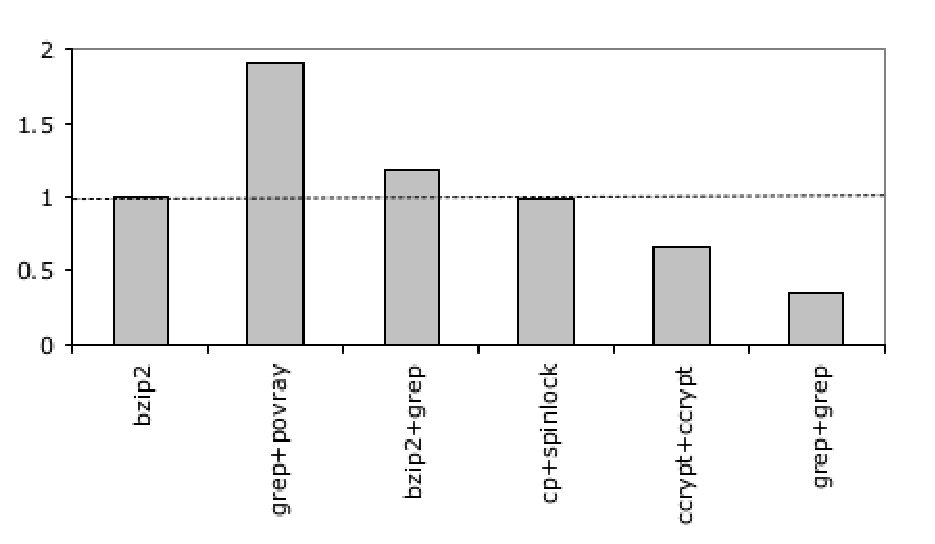
\includegraphics [keepaspectratio=true,scale=0.65]{figuras/interference_aplications.eps}
\caption{Variação de desempenho para combinações diferentes de aplicações}
\cite{koh2007}.
\label{interference_app}
\end{figure}

Além disso, é proposto por esse trabalho que com resultados desses desempenhos pode se fazer predição de desempenho de uma aplicação qualquer, a partir de análises matemáticas. Dado a quantidade variáveis, que são as métricas utilizadas para medição de desempenho, as análises matemáticas escolhidas foram a análise de componente principal e a análise de regressão linear. Um comparativo entre as análises foi feito de modo que chegou-se a conclusão que análise por PCA apresentava uma porcentagem de erro menor. Esse trabalho demonstrou que a taxa de erro utilizando o modelo PCA se manteve igual, mesmo utilizando outros servidores físicos com configurações diferentes. Entretanto, uma das restrições deste trabalho é que o mesmo fora aplicado em aplicações que estavam sendo executadas em duas máquinas virtuais. Desse modo como trabalhos futuros é proposta a investigação no uso de mais máquinas virtuais, e aplicação de modelos não lineares para predição de desempenho bem como a adição de novos tipos de métricas que envolvam outras características a nivel de sistema, tal como desempenho de aplicações de rede.

No trabalho de \citeonline{popiolek2012}, disserta sobre a importância de se utilizar métricas nativas (Tabela \ref{metric_tools}) de sistemas  operacionais tais como \textit{Linux} e \textit{Windows} para detecção de gargálos de performance. Esse trabalho acaba focando na aferição de operações de entrada e saída memória e uso de CPU, utilizando ferramentas de bencharmking para geração de cargas de trabalho. Seus cenários de teste são basicamente variando de uma a seis máquinas virtuais, sendo que o \textit{hypervisor} utilizado é o KVM. As análises permitem mostrar a queda de desempenho como um todo quando se tem o aumento do número de máquinas virtuais em em execução (Figura \ref{iobound_experiments}). Como trabalho futuros, propõe-se que sejam feitas análise estatísticas afim de comprovar possíveis relações entre as métricas observadas, alem de determinar o limiar que um sistema pode operar sem ter perda significativa no desempenho.

% Please add the following required packages to your document preamble:
% \usepackage{multirow}
\begin{table}[]
\centering
\caption{Contadores de desempenho de disco para \textit{Windows} e \textit{Linux} \cite{popiolek2012}}
\label{metric_tools}
\resizebox{1.0\textwidth}{!}{
\begin{tabular}{lllll}
\cline{1-4}
\multicolumn{1}{|l|}{Windows}                & \multicolumn{2}{l|}{Linux}                                             & \multicolumn{1}{c|}{\multirow{2}{*}{Descricao}}                                                                                                  &  \\ \cline{1-3}
\multicolumn{1}{|l|}{Monitor de Desempenho}  & \multicolumn{1}{l|}{iostat}          & \multicolumn{1}{l|}{df}         & \multicolumn{1}{c|}{}                                                                                                                            &  \\ \cline{1-4}
\multicolumn{1}{|l|}{\%Idle Time}            & \multicolumn{1}{l|}{-}               & \multicolumn{1}{c|}{-}          & \multicolumn{1}{c|}{\begin{tabular}[c]{@{}c@{}}Porcentagem de tempo\\  que o disco permanece inativo\end{tabular}}                               &  \\ \cline{1-4}
\multicolumn{1}{|l|}{(Disk Bytes/sec)/ 1024} & \multicolumn{1}{l|}{(rKB/s)+(wKB/s)} & \multicolumn{1}{c|}{-}          & \multicolumn{1}{c|}{\begin{tabular}[c]{@{}c@{}}Número de Kilobytes \\ lidos/escritos por segundo\end{tabular}}                                   &  \\ \cline{1-4}
\multicolumn{1}{|l|}{Disk Transfers/sec}     & \multicolumn{1}{l|}{(r/s)+(w/s)}     & \multicolumn{1}{c|}{-}          & \multicolumn{1}{c|}{\begin{tabular}[c]{@{}c@{}}Número de requisições\\  por segundo completadas\end{tabular}}                                    &  \\ \cline{1-4}
\multicolumn{1}{|l|}{Split IO/sec}           & \multicolumn{1}{c|}{-}               & \multicolumn{1}{c|}{-}          & \multicolumn{1}{c|}{\begin{tabular}[c]{@{}c@{}}Número de requisições por segundo\\  que foram divididas\\ em múltiplas requisições\end{tabular}} &  \\ \cline{1-4}
\multicolumn{1}{|l|}{Free Megabytes}         & \multicolumn{1}{c|}{-}               & \multicolumn{1}{l|}{Disponível} & \multicolumn{1}{c|}{\begin{tabular}[c]{@{}c@{}}Megabytes disponíveis para uso\\  em unidade de armazenamento\end{tabular}}                       &  \\ \cline{1-4}
\multicolumn{1}{|l|}{Avg. Disk sec/Transfer} & \multicolumn{1}{l|}{Await}           & \multicolumn{1}{c|}{-}          & \multicolumn{1}{l|}{Média de tempo para completar uma requisição}                                                                                &  \\ \cline{1-4}
\multicolumn{1}{|l|}{Avg. DIsk Queue Length} & \multicolumn{1}{l|}{avgqu-sz}        & \multicolumn{1}{c|}{-}          & \multicolumn{1}{c|}{\begin{tabular}[c]{@{}c@{}}Média de tamanho de filas de requisições\\  esperando pelo disco rígido\end{tabular}}             &  \\ \cline{1-4}
                                             &                                      &                                 &                                                                                                                                                  &  \\
                                             &                                      &                                 &                                                                                                                                                  &  \\
                                             &                                      &                                 &                                                                                                                                                  &  \\
                                             &                                      &                                 &                                                                                                                                                  &  \\
                                             &                                      &                                 &                                                                                                                                                  &  \\
                                             &                                      &                                 &                                                                                                                                                  &  \\
                                             &                                      &                                 &                                                                                                                                                  &  \\
                                             &                                      &                                 &                                                                                                                                                  & 
\end{tabular}}
\end{table}

\begin{figure}[!htb]
\centering
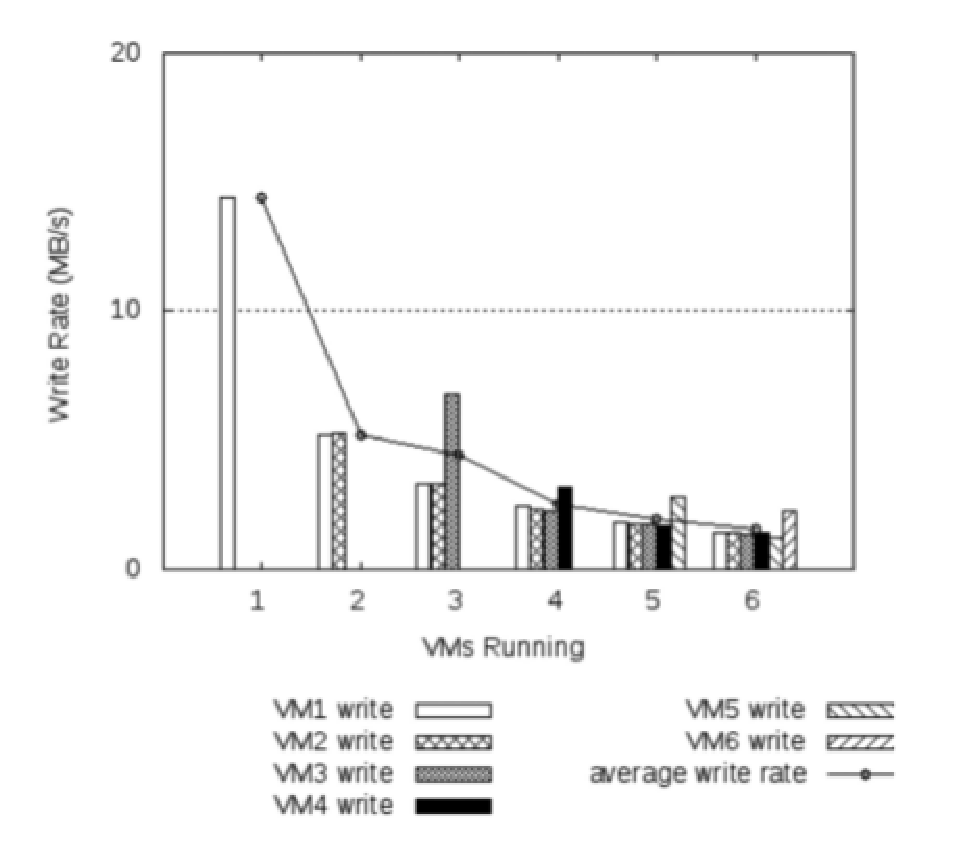
\includegraphics [keepaspectratio=true,scale=0.65]{figuras/iobound_experiments.eps}
\caption{Taxa de escrita em disco para experimentos voltados para E/S.}
\cite{popiolek2012}.
\label{iobound_experiments}
\end{figure}

Por fim, o trabalho de \citeonline{huber2011} tem como intuito prover um modelo genérico de predição de desempenho a partir de determinados fatores que podem interferir na virtualização(Figura \ref{influence_factors}). A idéia é que esse modelo genérico seja aplicável em diferentes tipos plataformas de virtualização. Assim, neste trabalho os experimentos são aplicados nos \textit{hypervisors } \textit{Citrix XenServer 5.5} e \textit{VMware ESX 4.0}. Os fatores categorizados para os experimentos foram: tipo de virtualização, configuração de gerenciamento de recursos e perfis de cargas de trabalho. Para o tipo de virtualização, os experimentos consistem em observar a perda de desempenha ocasionada com a virtualização. Na categoria de configuração de gerenciamento de recursos, são considerados fatores de configuração como número de máquinas virtuais e afinidade de núcleo. E para cargas de trabalho, foram executadas algumas ferramentas de \textit{benchmarking} a fim de se analisar diversas cargas de trabalho. Para o modelo de predição, fora utlizada análise de regressão linear assim como feito em \citeonline{koh2007}.

\begin{figure}[!htb]
\centering
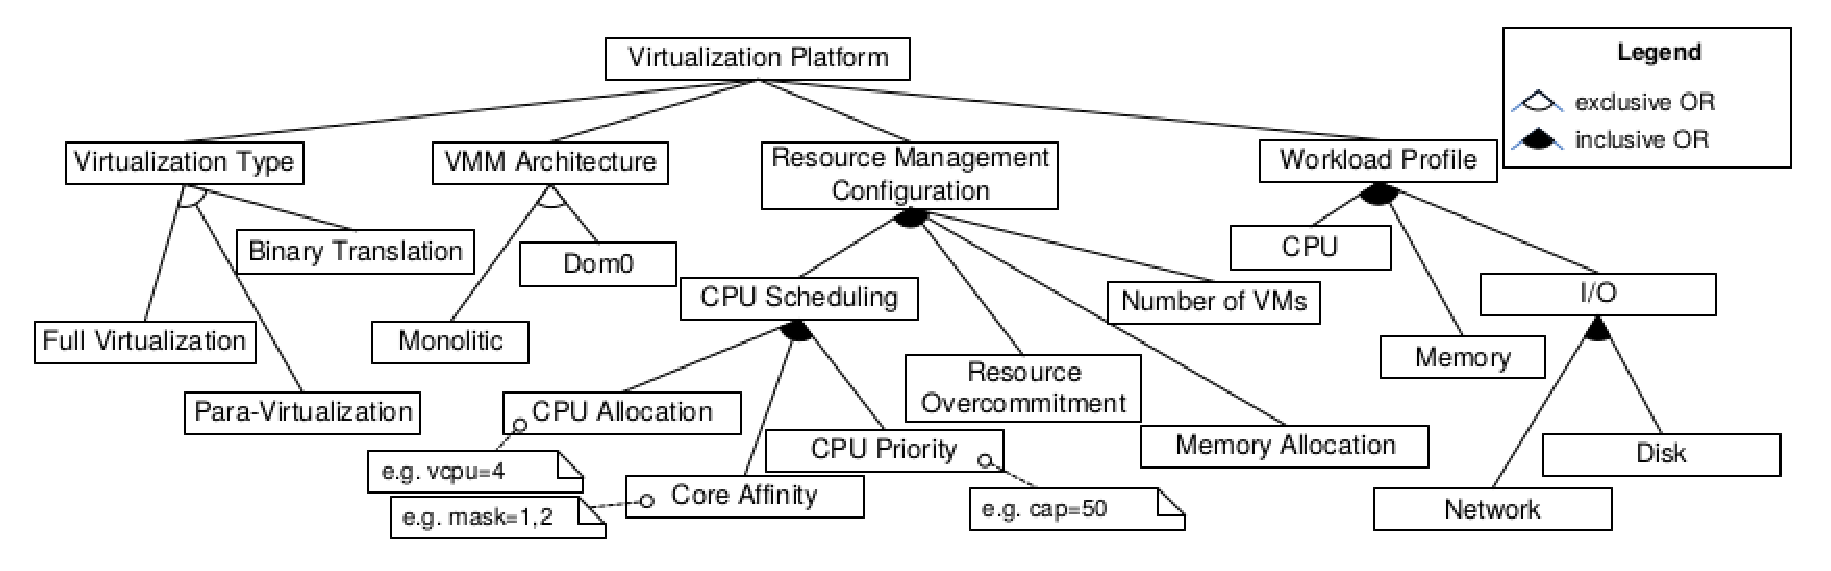
\includegraphics [keepaspectratio=true,scale=0.50]{figuras/factors_influence.eps}
\caption{Fatores que influenciam no desempenho de plataformas virtualizadas}
\cite{huber2011}.
\label{influence_factors}
\end{figure} 

Os trabalhos de \citeonline{koh2007} e \citeonline{huber2011} tem como ponto em comum o desenvolvimento de mecanismos que possam predizer o desempenho em ambientes virtualizados, uma característica interessante é que \citeonline{huber2011} aplica os mesmos experimentos em \textit{hypervisors} com arquiteturas distintas. Já o trabalho de \citeonline{koh2007} , apesar de fazer essa análise em apenas um \textit{hypervisor}, acaba focando na interferência que determinadas aplicações utilizadas no cotidiano, dependendo de sua característica a nivel de sistema, podem ocasionar em outras aplicações executadas em máquinas virtuais diferentes, no mesmo servidor físico,  trazendo assim um experimento mais próximo do que acontece no mundo real, tornando isso um diferencial deste trabalho. Desse modo, ainda com relação ao trabalho de \citeonline{koh2007}, um questionamento que poderia ser feito é com relação a aplicabilidade deste experimento em um outro \textit{hypervisor} com um tipo de virtualização diferente do apresentado no trabalho. Já o trabalho de \citeonline{popiolek2012} é mais voltado para monitoramento, análise de desempenho e detecção de gargalos a partir de métricas nativas do sistema operacional não sendo feito, como nos outros trabalhos, qualquer iniciativa de predição de desempenho.
\section{Questão problema}
Dado que o trabalho de \citeonline{koh2007} apresenta uma análise de interferência de desempenho utilizando o \textit{XEN}, que é um \textit{hypervisor} conhecido por utilizar a paravirtualização para provimento de máquinas virtuais, este trabalho visará responder a seguinte questão:

\textit{ Qual  grau de interferência entra máquinas virtuais, executando sob o mesmo servidor, utilizando o \textit{KVM} como \textit{hypervisor}, que implementa a virtualização total?  }
 
Tendo essa questão como ponto de referência, o objetivo deste trabalho é a aplicar um estudo de interferência entre máquinas virtuais, de modo que sejam comparados grau de interferência entre as duas técnicas de virtualização existentes: paravirtualização e virtualização total.
\subsection{Hipóteses}
A partir da questão problema definiu-se as seguintes hipóteses que irão motivar a realização deste trabalho:

\begin{itemize}
	\item \textit{H1}: O \textit{XEN}, por utilizar a paravirtualização como técnica de virtualização, apresenta menor interferência entre máquinas virtuais do que o \textit{KVM}.
	\item \textit{H2}: O modelo de predição proposto por \citeonline{koh2007} é aplicável em um ambiente com outro tipo de virtualização que não a provida pelo \textit{XEN}. %reformular
	\item \textit{H3}: Com esse mecanismo de predição de desempenho é possível propor uma nova distribuição de aplicações em um ambiente com múltiplas máquinas virtuais.  %reformular
\end{itemize}
	
\section{Ambiente de Testes}\label{sec:ambiente_teste}
Para o estudo proposto por este trabalho fora definido um  ambiente de testes que consiste no uso de máquinas virtuais com aplicações voltadas para realização
de testes de \textit{benchmark}. Tais aplicações foram definidas a partir do trabalho de \citeonline{koh2007}, tendo essas sido escolhidas visando o estresse de vários aspectos de sistema e de \textit{hardware}. Com a infraestrutura de computação em nuvem implementada com o \textit{OpenNebula} foi possível a criação desses ambientes de testes em máquinas virtuais criadas remotamente. As máquinas virtuais possuíam, como configuração, sistema operacional \textit{Centos 7}, espaço em disco de 15GB e 1GB de memória \textit{RAM}. Em um primeiro momento as aplicações foram instaladas e testadas de modo que se pudesse observar quais são os comandos utilizados para funcionamento das mesmas, em seguida foram criados \textit{snapshots} das máquinas virtuais com o auxílio provido pelo \textit{OpenNebula}. 

Assim era possível criar, destruir e efetuar quaisquer tipos de testes com relativa comodidade. Entre as aplicações escolhidas estão típicas provedoras de \textit{stress} computacional no cotidiano tais como compilação de código fonte, compressão e criptação de arquivos e rendenrização de \textit{frames}. Há também ferramentas voltadas para geração de testes de \textit{benchmark} tais como \textit{Cachebench} e \textit{AIM Benchmark suite}. A seguir é feita uma breve descrição das ferramentas utilizadas.

\begin{itemize}
\item \textit{Add\_double} é um dos vários programas de testes de carga existentes no \textit{AIM benchmark suite}. É responsável por medir operações de adição de dupla precisão.

\item \textit{Bzip2} e \textit{Gzip} são aplicações típicas para compressão e descompressão de arquivos. Para realização de testes de compressão fora definido o uso de arquivos com tamanho no mínimo o dobro da memória \textit{RAM}, assim utilizou-se arquivos com tamanho de 3GB. Evitando assim o efeito de \textit{cache} de grande parte desse arquivo na memória.

\item \textit{Ccrypt} é uma ferramenta de código aberto voltada para encriptação e desencriptação de arquivos. Foi desenvolvido com o intuito de substituir a aplicação padrão do \textit{unix}, o \textit{crypt} \cite{ccrypt}.

\item \textit{Cachebench} é uma ferramenta de \textit{benchmark} de código aberto desenvolvida para avaliar o desempempenho do subsistema de memória. Atualmente é integrado \textit{LLCbench} (\textit{Low-Level Characterization Benchmarks}) \cite{cachebench}.

\item \textit{Cat} e \textit{Grep} são comandos padrões em sistemas \textit{Linux} que são responsáveis por gerar requisições de leitura no disco. \textit{Cat} é reponsável por mostrar conteúdo de arquivos bem como combina-los e criar outros novos. Enquanto que \textit{Grep} é utilizado para busca de palavras em arquivos texto.

\item \textit{cp} e \textit{dd} são outros comandos padrões em sistemas \textit{Linux}, neste caso, responsáveis por gerar atividades voltadas para escrita de disco. \textit{cp} é utilizado para copiar arquivos e diretórios. O comando \textit{dd} é utilizado para criação de imagens e cópias de arquivos.

\item \textit{Iozone} é uma ferramenta de \textit{benchmark} utilizada, voltada para testes de operações de disco, tais como leitura e escrita \cite{iozone}.

\item \textit{Bw\_mem} é umas das ferramentas de \textit{benchmark}, voltada para testes de leitura e escrita de memória, que compôem o \textit{LMbench} \cite{lmbench}.

\item \textit{Make} é um comando nativo em sistemas operacionais \textit{Linux}, responsável por automatizar um conjunto de procedimentos, principalmente  a compilação de programas grandes que possuem vários arquivos com códigos fontes. 

\item \textit{Povray} é uma ferramenta de codigo aberto voltada para para renderização de quadros com gráficos 3-D \cite{povray}.

\end{itemize}

Além das ferramentas já mostradas outras aplicações foram utilizadas no trabalho de \textit{koh2007}: \textit{Spinlock}, \textit{CacheBuster} e \textit{Analyser}.

\section{Coleta de dados} 
Dada a configuração do servidor apresentado na seção \ref{sec:infraestrutura}, um dos receios era de que os testes de \textit{benchmark} feitos não fossem suficientes para apresentarem interferência entre as máquinas virtuais, desse modo optou-se por dividr a coleta de dados em três experimentos práticos de modo que, nos dois primeiros experimentos fossem verificadas as interferências entre os diversos tipos de aplicações. Assim, para cada experimento foi definido objetivos específicos a serem alcançados.
%A coleta de dados foi efetuada a apartir da realização de três experimentos práticos. Para cada experimento foi definido objetivos específicos a serem alcançados.%

O primeiro experimento tinha como objetivo verificar a existência da interferência entre máquinas virtuais no servidor físico utilizado, sendo neste experimento executado com poucas ferramentas dado que os resultados eram mais voltados para verificação da interferência e motivação da continuidade do trabalho em si do que para uma análise mais profunda. No segundo experimento, teve como objetivo verificar a variação de interferência para o conjunto completo das ferramentas já apresentadas. No terceiro experimento, teve como foco a avaliação da interferência para diversos tipos de caracteristicas a níveis de sistema tais como média de utilização de \textit{CPU} e \textit{leitura e escrita de disco por segundo}, por exemplo. Sendo os resultados deste terceiro e último experimentos utilizados como insumo para análise de dados apresentada neste trabalho. A amostragem dos dados referentes a cada experimento foi baseada nos resultados apresentados no trabalho de \citeonline{koh2007}, visando assim um comparativo dos resultados encontrados.

\subsection{Cálculo da Interferência}
Os procedimentos adotados para o cálculo da interferência seguem os propostos no trabalho de \citeonline{koh2007}. Desse modo, duas máquinas virtuais, com as especificações e aplicações de \textit{benchmark} apresentadas na seção \ref{sec:ambiente_teste}, são criadas em um servidor utilizando \textit{hypervisor} \textit{KVM}. Cada máquina virtual, denominadas \textit{'dom1'} e \textit{'dom2'} respectivamente, executa uma das aplicações de \textit{benchmarking}. Uma aplicação executando em \textit{dom1} é chamada de aplicação \textit{foreground}, e a que estiver executando em \textit{dom2} é a aplicação \textit{background}. 
\subsection{Características de Cargas de trabalho a nível de sistema}


\section{Análise de dados}
Análise estatística
Variável independente
variável dependente
Análise multivariada
 	